\documentclass{beamer}

%
% Choose how your presentation looks.
%
% For more themes, color themes and font themes, see:
% http://deic.uab.es/~iblanes/beamer_gallery/index_by_theme.html
%
\mode<presentation>
{
  \usetheme{default}      % or try Darmstadt, Madrid, Warsaw, ...
  \usecolortheme{default} % or try albatross, beaver, crane, ...
  \usefonttheme{default}  % or try serif, structurebold, ...
  \setbeamertemplate{navigation symbols}{}
  \setbeamertemplate{caption}[numbered]
  \setbeamertemplate{footline}[page number]
  \setbeamercolor{frametitle}{fg=white}
  \setbeamercolor{footline}{fg=black}
} 

\usepackage[english]{babel}
\usepackage[utf8x]{inputenc}
\usepackage{tikz}
\usepackage{listings}
\usepackage{courier}

\xdefinecolor{darkblue}{rgb}{0.1,0.1,0.7}
\xdefinecolor{dianablue}{rgb}{0.18,0.24,0.31}
\definecolor{commentgreen}{rgb}{0,0.6,0}
\definecolor{stringmauve}{rgb}{0.58,0,0.82}

\lstset{ %
  backgroundcolor=\color{white},      % choose the background color
  basicstyle=\ttfamily\small,         % size of fonts used for the code
  breaklines=true,                    % automatic line breaking only at whitespace
  captionpos=b,                       % sets the caption-position to bottom
  commentstyle=\color{commentgreen},  % comment style
  escapeinside={\%*}{*)},             % if you want to add LaTeX within your code
  keywordstyle=\color{blue},          % keyword style
  stringstyle=\color{stringmauve},    % string literal style
  showstringspaces=false,
  showlines=true
}

\lstdefinelanguage{scala}{
  morekeywords={abstract,case,catch,class,def,%
    do,else,extends,false,final,finally,%
    for,if,implicit,import,match,mixin,%
    new,null,object,override,package,%
    private,protected,requires,return,sealed,%
    super,this,throw,trait,true,try,%
    type,val,var,while,with,yield},
  otherkeywords={=>,<-,<\%,<:,>:,\#,@},
  sensitive=true,
  morecomment=[l]{//},
  morecomment=[n]{/*}{*/},
  morestring=[b]",
  morestring=[b]',
  morestring=[b]"""
}

\title[2016-08-18-focus-group-advertisement]{Computing for Data Analysis}
\author{Jim Pivarski}
\institute{Princeton University -- DIANA}
\date{August 18, 2016}

\begin{document}

\logo{\pgfputat{\pgfxy(0.11, 8)}{\pgfbox[right,base]{\tikz{\filldraw[fill=dianablue, draw=none] (0 cm, 0 cm) rectangle (50 cm, 1 cm);}}}\pgfputat{\pgfxy(0.11, -0.6)}{\pgfbox[right,base]{\tikz{\filldraw[fill=dianablue, draw=none] (0 cm, 0 cm) rectangle (50 cm, 1 cm);}
\includegraphics[height=0.99 cm]{diana-hep-logo.png}\tikz{\filldraw[fill=dianablue, draw=none] (0 cm, 0 cm) rectangle (4.9 cm, 1 cm);}}}}

\begin{frame}
  \titlepage
\end{frame}

\logo{\pgfputat{\pgfxy(0.11, 8)}{\pgfbox[right,base]{\tikz{\filldraw[fill=dianablue, draw=none] (0 cm, 0 cm) rectangle (50 cm, 1 cm);}
\includegraphics[height=1 cm]{diana-hep-logo.png}}}}

% Uncomment these lines for an automatically generated outline.
%\begin{frame}{Outline}
%  \tableofcontents
%\end{frame}

\begin{frame}{What I've been up to}
\vspace{0.5 cm}
\begin{itemize}\setlength{\itemsep}{0.25 cm}
\item Finding ways to export HEP data to Machine Learning (ML) and Big Data (BD) platforms.
\begin{itemize}
\item ML: {\it Numpy, Pandas, Keras, Theano, Scikit-Learn, R.} \\ Training MVAs, often Python or R, often on GPUs.
\item BD: {\it Spark, Hadoop, Drill, Pig, Impala.} \\ Simplifying distributed computing, often in Java/Scala (JVM).
\end{itemize}
\item Developing a histogram abstraction for more versitile and portable data analysis.
\item Planning projects to develop low-latency (``no ntuple'') physics analysis servers.
\item Planning studies of physicists' needs and interests in computing for data analysis.
\item Strengthening connections with developers in industry.
\end{itemize}
\end{frame}

\begin{frame}{What this means for you}
\begin{itemize}\setlength{\itemsep}{0.5 cm}
\item Is there an ML/BD tool from industry you'd like to learn more about? I can give workshops at the LPC.
\item When my software products are in a mature state (some of them are), I can give workshops on those and show how they enable access to ML/BD tools.
\item I want to run a focus group to learn your opinions. \\ If you qualify, please sign up!
\end{itemize}
\end{frame}

\begin{frame}{Focus group!}
\vspace{0.25 cm}
\begin{description}
\item[Definition:]<1-> a means of collecting opinion data that is more open to the unexpected than surveys.
\item[Method:]<2-> at most 10 interested physicists would meet with me for an hour to discuss a list of prepared questions. Conversations are private and anonymous but would result in a consensus statement. If more than 10 are interested, I'll run two identical sessions.
\item[Topic:]<3-> usefulness of new computing techniques in data analysis: the cost/benefit analysis you use to judge the value of learning something new.
\item[Target group:]<4-> physicists {\it performing data analysis,} meaning ``hands on the keyboard,'' as opposed to directing an analysis group. Typically graduate students and postdocs.
\end{description}

\uncover<5->{Results of this study (and other identical sessions) would contribute to a community whitepaper for the NSF's (SI)$^2$ project.}
\end{frame}

\begin{frame}{Workshops}
\vspace{0.5 cm}
\begin{itemize}\setlength{\itemsep}{0.75 cm}
\item In the spring, I led a walkthrough of using Apache Spark and Scala (Spark's native language) for Matteo Cremensi, Cristina Suarez, and several others.

\vspace{0.25 cm}
Matteo and Cristina have since ported their analysis (a {\it lot} of C++ code) to Scala.

\vspace{0.25 cm}
(Note: this is not the only way to do it.)

\item I'm willing to lead sessions on
\begin{itemize}
\item ML/BD technologies you're casually interested in (overviews).
\item ML/BD technologies you intend to use (in-depth dives, assuming we have a way to get your data into it).
\item my own software, which is generally intended to enable the above.
\end{itemize}
\end{itemize}
\end{frame}

\begin{frame}{}
\begin{center}
\Huge \textcolor{darkblue}{Potential topics of interest}
\end{center}
\end{frame}

\begin{frame}{Transferring/translating data for ML/BD}
\vspace{0.5 cm}
\begin{block}{Many alternatives are being considered:}
\begin{enumerate}
\item Direct write from CMSSW to an ML/BD-friendly file format (no ROOT).
\item Conversion of ROOT to an intermediate file format.
\item Accessing ROOT in ML/BD applications: embedded or forked process.
\end{enumerate}
\end{block}

\vspace{-0.25 cm}
\begin{block}{Presently available:}
\begin{enumerate}
\item \textcolor{darkblue}{c2numpy}: write (flat) Numpy files from C/C++.
\item \textcolor{darkblue}{root2avro}: convert (complex) TTrees to Avro files.
\item \textcolor{darkblue}{ScaROOT-Reader}: read (complex) TTrees in Scala and Spark, embedded and forked.
\end{enumerate}
\end{block}

\vspace{-0.25 cm}
\begin{block}{Future:}
Conversion from ROOT to {\it anything} through Apache Arrow.
\end{block}
\end{frame}

\begin{frame}{c2numpy}
\vspace{0.5 cm}
Extremely simple, no dependencies, just a header file.

\vspace{0.25 cm}
C/C++ processes can write flat ntuples Numpy's native format, and therefore {\it Pandas, Keras, Theano, Scikit-Learn, etc.}

\begin{center}
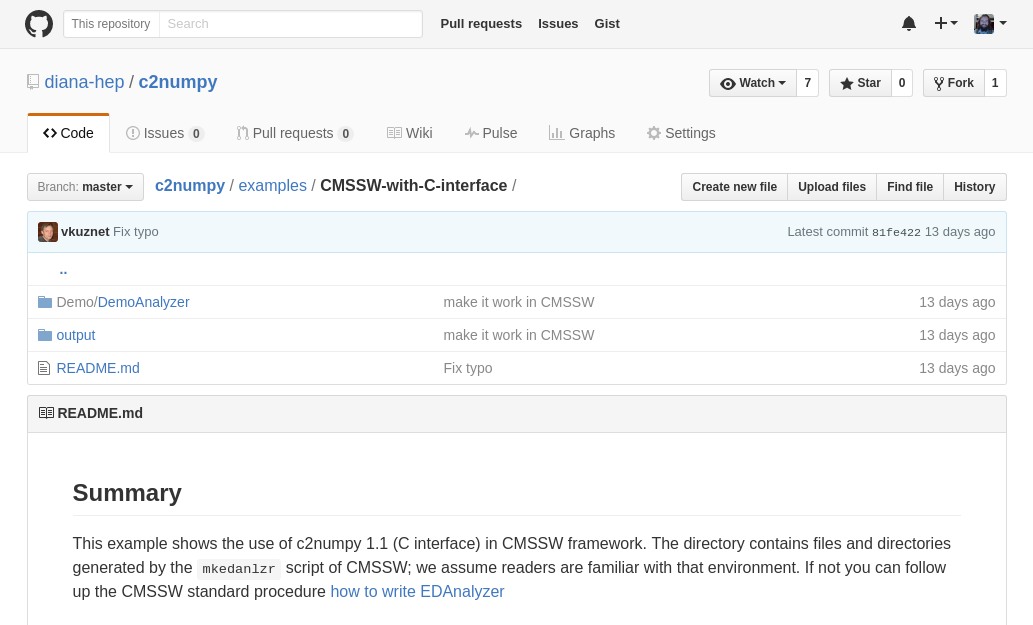
\includegraphics[width=0.9\linewidth]{c2numpy.png}
\end{center}
\end{frame}

\begin{frame}{root2avro and ScaROOT-Reader}
\vspace{0.5 cm}
\begin{columns}
\column{0.7\linewidth}
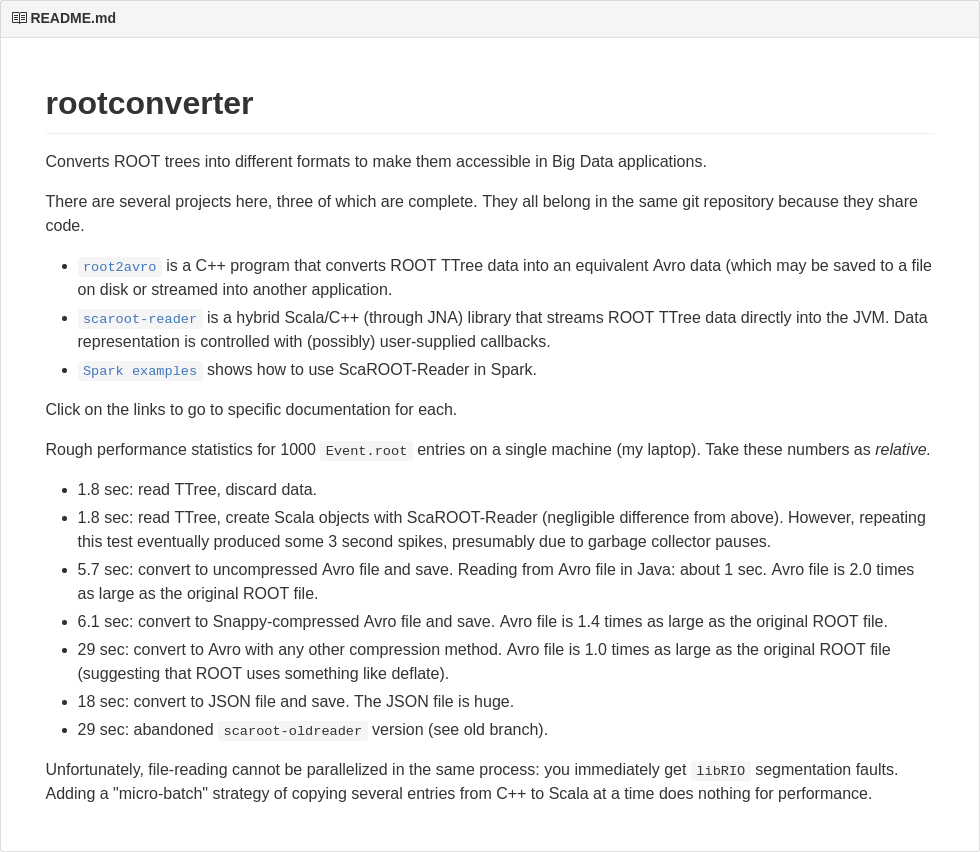
\includegraphics[width=\linewidth]{rootconverter.png}

\column{0.3\linewidth}
GitHub repo:
\textcolor{darkblue}{diana-hep/rootconverter}

\vspace{0.5 cm}
Three converters:

\vspace{0.2 cm}
\textcolor{darkblue}{root2avro}: \\
\hspace{0.25 cm} standalone \\
\hspace{0.25 cm} converter

\vspace{0.2 cm}
\textcolor{darkblue}{ScaROOT-Reader}: \\
\hspace{0.25 cm} direct ROOT $\to$ \\
\hspace{0.25 cm} Scala, embedded \\
\hspace{0.25 cm} and forked
\end{columns}
\end{frame}

\begin{frame}{Future: ROOT $\to$ Apache Arrow $\to$ anything}
\vspace{0.25 cm}
\begin{center}
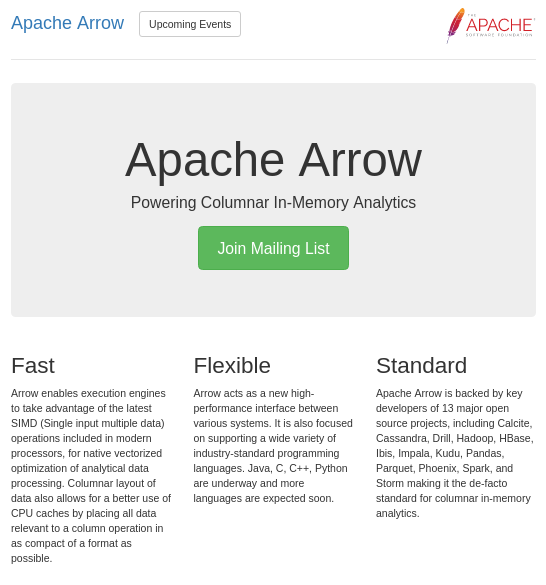
\includegraphics[width=0.7\linewidth]{arrow.png}
\end{center}
\end{frame}

\begin{frame}{Apache Arrow}
\begin{block}{In-memory representation of abstract types}
\begin{itemize}
\item Standard numbers, strings, structs, arrays/maps (immutable).
\item Not a file format: {\it in-memory} (but closely aligned to Parquet).
\item Major ML/BD packages are being rewritten to perform calculations on data in this form.
\item Zero-copy sharing of data among C++, Python, R, JVM.
\end{itemize}
\end{block}

\vspace{0.5 cm}
\mbox{\hspace{-0.25 cm}\begin{minipage}{1.05\linewidth}
\begin{columns}
\column{0.45\linewidth}
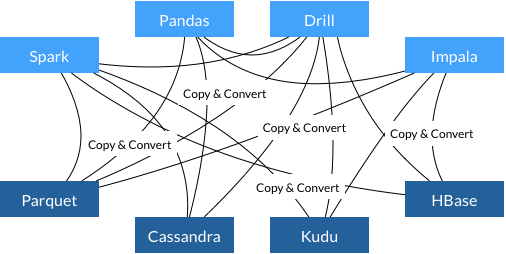
\includegraphics[width=\linewidth]{copy2.png}

\column{0.01\linewidth}
\centering $\to$

\column{0.45\linewidth}
\only<1>{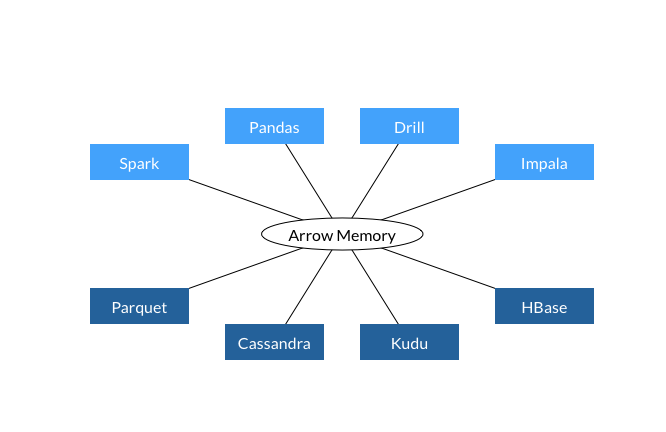
\includegraphics[width=\linewidth]{shared2.png}}\only<2>{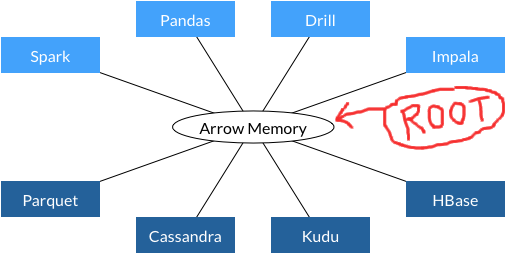
\includegraphics[width=\linewidth]{shared3.png}}
\end{columns}
\end{minipage}}
\end{frame}

\begin{frame}{Apache Arrow}
\vspace{0.5 cm}
Pandas, Spark, and BD SQL engines (notably Drill) are refactoring to process data as contiguous columns to optimize use of CPU cache, a.k.a.\ ``vectorizing'' their code.

\vspace{0.5 cm}
\begin{columns}
\column{0.7\linewidth}
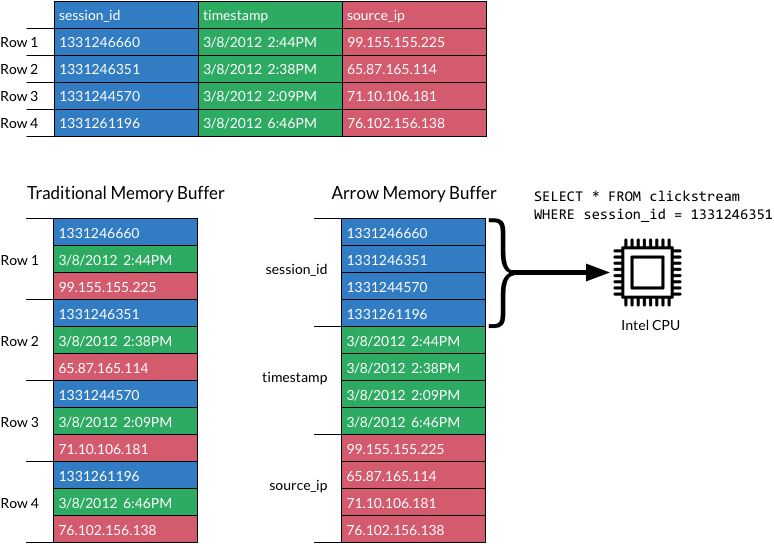
\includegraphics[width=\linewidth]{simd.png}

\column{0.3\linewidth}
RAM $\to$ CPU cache benefit is analogous to disk $\to$ RAM benefit of columnar data access.

\vspace{0.5 cm}
Since they're refactoring anyway, they chose to do so in a common way.
\end{columns}
\end{frame}

\begin{frame}{Histogrammar}
\vspace{0.25 cm}
\fbox{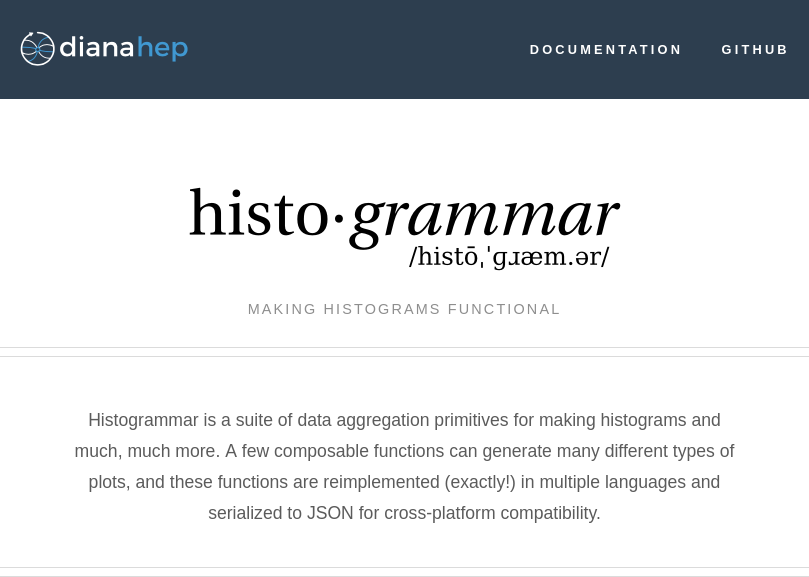
\includegraphics[width=0.8\linewidth]{histogrammar1.png}}

\vspace{-2.7 cm}
\textcolor{blue}{\small \url{http://histogrammar.org}} \hfill 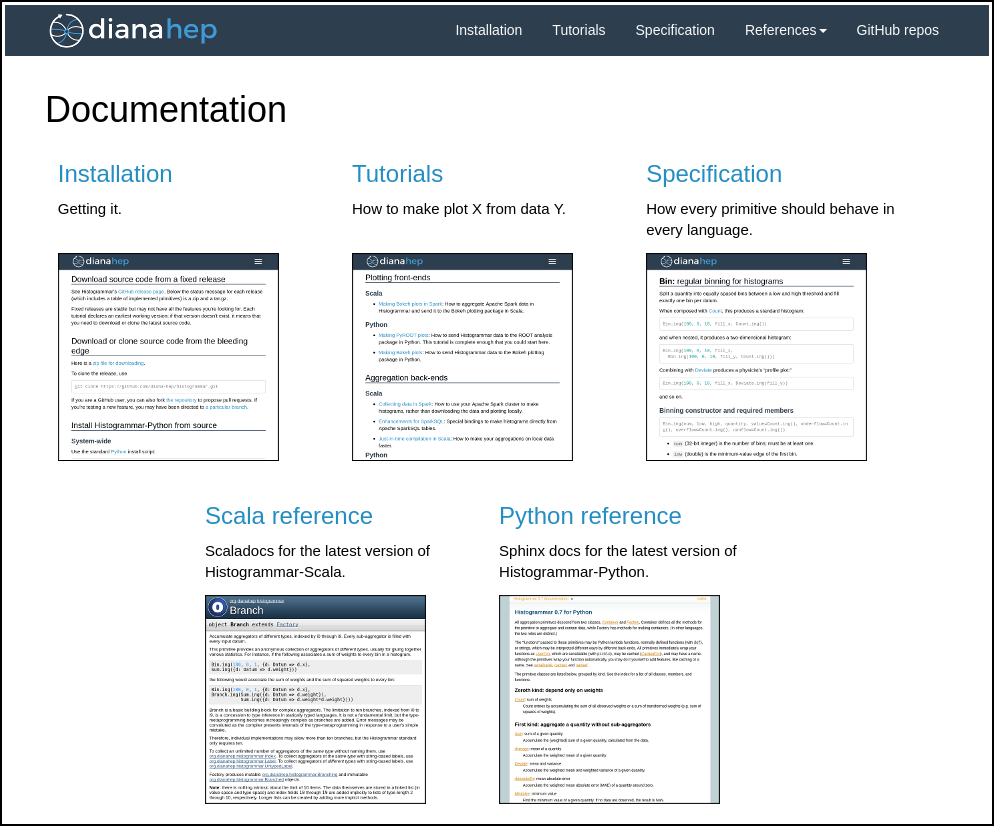
\includegraphics[width=0.5\linewidth]{histogrammar2.png}
\end{frame}

\begin{frame}{Histogrammar}
\vspace{0.5 cm}
\begin{itemize}\setlength{\itemsep}{0.25 cm}
\item Motivated by the need to match Spark's way of aggregating data (scatter-gather) with the HBOOK/PAW/ROOT way (histogram is a fillable container).

\begin{center}
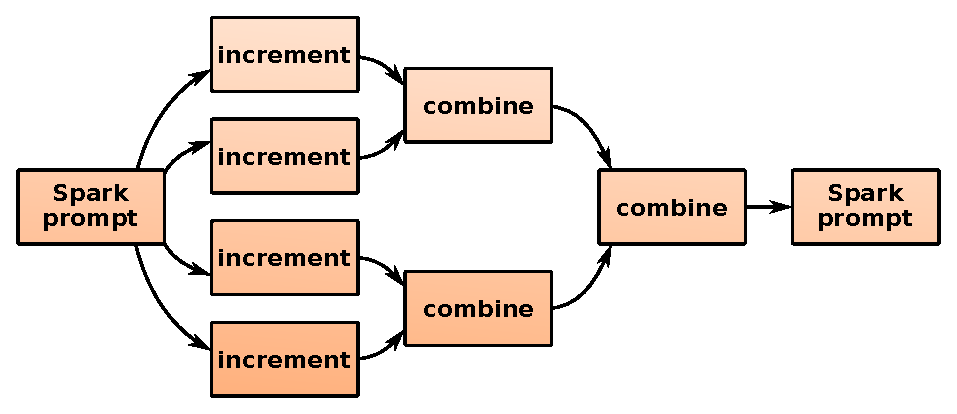
\includegraphics[width=0.7\linewidth]{aggregate.pdf}
\end{center}

\item A 20-primitive ``language'' of aggregation that covers all common histogram types and potentially new ones.

\item Parallelization is built-in (primitives and any composition of them are associative and commutative).
\end{itemize}
\end{frame}

\begin{frame}{You can benefit now}
\vspace{0.25 cm}

\only<1>{Contains hooks to fill ROOT histograms from ROOT TTrees {\it in Python as fast as C++.}}

\only<2>{Replace a suite of {\small \tt ntuple.Draw} commands or a Python {\small \tt for} loop for a dramatic speed-up. Leave the rest of the analysis in ROOT.}

\renewcommand{\arraystretch}{1.2}
\vspace{0.25 cm}
\mbox{\hspace{-0.5 cm}
\fbox{\begin{tabular}{l c c c c}
\textcolor{darkblue}{ROOT} & & & & \\
Fill method & Preparation & Prep (ms) & Run (ms) & Relative \\\hline
C++ & compilation & 12.6 & \textcolor{red}{198} & \textcolor{red}{1} \\
PyROOT & none & & 15,700 & 79 \\
TFormula & first pass & 380 & 317 & 1.6\vspace{0.25 cm} \\
\textcolor{darkblue}{Histogrammar} & & & & \\
Fill method & Preparation & Prep (ms) & Run (ms) & Relative \\\hline
pure Python & none & & 21,000 & 105 \\
with Numpy & first pass & 814 & 312 & 1.6 \\
with ROOT & JIT-compilation & 219 & \textcolor{red}{196} & \textcolor{red}{0.98} \\
\end{tabular}}}
\end{frame}

\begin{frame}{Future directions of Histogrammar}
\vspace{0.5 cm}
\begin{itemize}\setlength{\itemsep}{0.2 cm}
\item Using Histogrammar to plot data in GPUs (soon: 1--2 weeks).
\item GPU-enabled server for instant plotting of large datasets (later: 1--2 years).
\item Integration into ROOT 6 (Python-only) and ROOT 7 (C++).
\end{itemize}

\vspace{1 cm}
\pgfputat{\pgfxy(20, 0)}{\pgfbox[right,base]{\tikz{\filldraw[fill=dianablue, draw=none] (0 cm, 0 cm) rectangle (50 cm, 1 cm);}}}

\vspace{-0.35 cm}
\hspace{-0.83 cm} \textcolor{white}{\Large Targeting both physicists and data scientists}

\vspace{0.35 cm}
\begin{itemize}\setlength{\itemsep}{0.2 cm}
\item Workshops and one-on-one help to integrate Histogrammar into your analyses.
\item Also presenting it to data scientists:
\begin{itemize}
\item StrangeLoop conference, September 15--16.
\item Chicago Hadoop User's Group (CHUG), October TBD.
\end{itemize}
\item Cross-cultural! Data scientists don't use plotting as much as they should\ldots
\end{itemize}
\end{frame}

\begin{frame}{More cross-cultural integration}
\vspace{0.5 cm}
\begin{columns}
\column{0.5\linewidth}
Data scientists use declarative (order-independent) queries to compute high-level quantities efficiently.

\vspace{0.25 cm}
Example: breaking up SQL into work-plans, organizing data access to avoid CPU cache misses.

\column{0.5\linewidth}
Physicists perform more complex queries than can be (easily) expressed in SQL.

\vspace{0.25 cm}
But still, access patterns are fairly regular: rarely correlate data between events, filter-maximize-cut, match reco/gen particles\ldots
\end{columns}

\begin{uncoverenv}<2->
\vspace{-0.5 cm}
\[ \underbrace{\mbox{\hspace{10 cm}}}{} \]

\begin{itemize}
\item Introduce new, HEP-friendly primitives to declarative languages?
\item I've discussed this with a senior Spark contributor and a lead Pandas developer.
\begin{itemize}
\item ``Our students want new structures to optimize.''
\item ``Maybe a post-1.0 Pandas version should cover these.''
\end{itemize}
\end{itemize}
\end{uncoverenv}
\end{frame}

\begin{frame}{Building connections with ML/BD community}

\begin{itemize}\setlength{\itemsep}{0.5 cm}
\item KDD conference in San Francisco (yesterday).
\item Promoting Histogrammar at StrangeLoop and CHUG to encourage contributions from industry.
\item I may be contributing HEP-relevant code to Apache Arrow.
\item Spark, Parquet, Arrow developer's forums.
\item Conversations with some famous people (name dropping).
\end{itemize}
\end{frame}

\begin{frame}{}
\begin{center}
\textcolor{darkblue}{\Huge Sign up for the focus group!}

\vspace{1 cm}
\Large I want your opinions!
\end{center}
\end{frame}

\end{document}
